% \documentclass[9pt,a4paper,twocolumn,landscape,oneside]{amsart}
\documentclass[8pt,a4paper,landscape,oneside]{amsart}
\usepackage{amsmath, amsthm, amssymb, amsfonts}
\usepackage[T1]{fontenc}
\usepackage[utf8]{inputenc}
\usepackage{booktabs}
\usepackage{fancyhdr}
\usepackage{float}
\usepackage{fullpage}
%\usepackage{geometry}
\usepackage[landscape]{geometry}
% \usepackage{listings}
\usepackage{caption, subcaption}
\usepackage[scaled]{beramono}
\usepackage{color,graphicx,overpic}
\usepackage{titling}
\usepackage{datetime}
\usepackage{multicol}
\usepackage{calc}
\usepackage{ifthen}
\usepackage{hyperref}
\usepackage{environ}
\usepackage{tabularx}
\usepackage[dvipsnames]{xcolor}


% Minted (For code stuff)
\usepackage{minted}
\newcommand{\code}[1]{\inputminted[fontsize=\footnotesize]{c}{#1}}

% This sets the margins to .5cm
\geometry{top=0pt,left=.3cm,right=.3cm,bottom=1cm}

\setlength{\headheight}{15.2pt}
\renewcommand{\headrulewidth}{0.4pt}
\renewcommand{\footrulewidth}{0.4pt}

% Turn off header and footer
% \pagestyle{empty}

% Redefine section commands to use less space
\makeatletter
\renewcommand{\section}{\@startsection{section}{1}{0mm}%
                                {-1ex plus -.5ex minus -.2ex}%
                                {0.5ex plus .2ex}%x
                                {\normalfont\large\bfseries}}
\renewcommand{\subsection}{\@startsection{subsection}{2}{0mm}%
                                {-1explus -.5ex minus -.2ex}%
                                {0.5ex plus .2ex}%
                                {\normalfont\normalsize\bfseries}}
\renewcommand{\subsubsection}{\@startsection{subsubsection}{3}{0mm}%
                                {-1ex plus -.5ex minus -.2ex}%
                                {1ex plus .2ex}%
                                {\normalfont\small\bfseries}}
\makeatother


% Don't print section numbers
\setcounter{secnumdepth}{0}


\setlength{\parindent}{0pt}
\setlength{\parskip}{0pt plus 0.5ex}

\newcommand{\subtitle}[1]{%
  \posttitle{%
    \par\end{center}
    \begin{center}\large#1\end{center}
    \vskip0.5em}%
}

% Header/Footer
% \geometry{includeheadfoot}
% \fancyhf{}
\pagestyle{fancy}
\lhead{HSR}
\rhead{Silvan Adrian\quad\thepage}
\cfoot{}

% Title/Author
\title{WED1 Cheat Sheet}
\subtitle{}
\date{\ddmmyyyydate{\today{}}}

% Output Verbosity
\newif\ifverbose
\verbosetrue
% \verbosefalse

% Some list helpers from graph theory
\newcounter{temp}
\newcounter{ilist_counter}
\newcounter{iilist_counter}

\newenvironment{ilist}{
  \begin{list}{{\bf \arabic{ilist_counter}}}{
      \usecounter{ilist_counter}
      \addtolength{\labelsep}{.6ex}
      \addtolength{\itemsep}{1ex}
      \setlength{\leftmargin}{1.4em}}
    %   \setcounter{ilist_counter}{\value{temp}}
}{
%   \setcounter{temp}{\value{ilist_counter}}
  \end{list}
}

\newenvironment{iilist}{
  \begin{list}{{\bf \alph{iilist_counter}}}{
      \usecounter{iilist_counter}
      \addtolength{\labelsep}{.6ex}
      \addtolength{\itemsep}{.5ex}
      \setlength{\leftmargin}{1.7em}}
}{
  \end{list}
}

\newenvironment{iblist}{
  \begin{list}{{\bf $\bullet$}}{
      \addtolength{\labelsep}{.6ex}
      \addtolength{\itemsep}{.5ex}
      \setlength{\leftmargin}{1.7em}}
}{
  \end{list}
}

% Theorems and solutions
\theoremstyle{plain}
\newtheorem{theorem}{Theorem}
\newtheorem*{theorem*}{Theorem}
\newtheorem{corollary}[theorem]{Corollary}
\newtheorem*{corollary*}{Corollary}
\newtheorem{lemma}[theorem]{Lemma}
\newtheorem*{lemma*}{Lemma}
\newtheorem{proposition}[theorem]{Proposition}
\newtheorem*{proposition*}{Proposition}
\newtheorem{conjecture}[theorem]{Conjecture}
\newtheorem*{conjecture*}{Conjecture}
\newtheorem*{solution}{Solution}

\theoremstyle{definition}
\newtheorem{definition}[theorem]{Definition}
\newtheorem*{definition*}{Definition}
\newtheorem{example}[theorem]{Example}
\newtheorem*{example*}{Example}
\newtheorem{problem}[theorem]{Problem}
\newtheorem*{problem*}{Problem}

\theoremstyle{remark}
\newtheorem{remark}{Remark}
\newtheorem*{remark*}{Remark}

% For writing vectors
\let\oldhat\hat
\let\oldvec\vec
\renewcommand{\vec}[1]{\oldvec{\mathbf{#1}}}
\newcommand{\vecb}[1]{\mathbf{#1}}
\renewcommand{\hat}[1]{\oldhat{\mathbf{#1}}}

\newcommand{\cvect}[2]{ \begin{pmatrix} #1 \\ #2 \end{pmatrix} }
\newcommand{\ctvect}[3]{ \begin{pmatrix} #1 \\ #2 \\ #3 \end{pmatrix} }
\newcommand{\vect}[2]{ \langle #1 , #2 \rangle }
\newcommand{\tvect}[3]{ \langle #1 , #2 , #3 \rangle }
\newcommand{\qvect}[4]{ \langle #1 , #2 , #3 \rangle }

% For equations
\NewEnviron{formula}{
    \abovedisplayshortskip=0pt
    \belowdisplayshortskip=0pt
    \abovedisplayskip=0pt
    \belowdisplayskip=0pt
    \begin{align*}
        \BODY
    \end{align*}
}
\newcommand{\eqn}[1]{\begin{formula} #1 \end{formula}}
% The actual document

\newcounter{line}
\newcolumntype{C}{>{\ttfamily\arraybackslash}l}
\newcolumntype{E}{>{\ttfamily\arraybackslash}c}
\newcolumntype{R}{>{\ttfamily\arraybackslash}r}
\newcolumntype{b}{>{\bfseries\arraybackslash}l}
\newenvironment{tabularlc}[1]{
\setcounter{line}{0}
\begin{tabular}{#1}
}{
\end{tabular}
}
\newenvironment{ldesc}{
\begin{tabularlc}{lC}
}{
\end{tabularlc}
}
\newenvironment{Ldesc}{
\begin{ldesc}
\hline
}{
\\\hline
\end{ldesc}
}
\newcommand{\C}{\texttt}
\newcommand{\B}{\textbf}
\newcommand{\I}{\textit}
\newcommand{\CI}[1]{\texttt{\textit{#1}}}
\newcommand{\N}{\textnormal}
\newcommand{\T}[1]{\hphantom{\I{#1}}}
\newcommand{\D}[1]{\hphantom{#1}}
\newcommand{\lditem}[2]{
	#1 & #2 \\
}
\newcommand{\li}[1][]{%
\stepcounter{line}%
\ifnum\theline>1 \\\fi%
#1 &
}
\newcommand{\lI}[1][]{%
\stepcounter{line}%
\ifnum\theline>1 \\[1ex]\fi%
#1 &
}
\newcommand{\Li}[1][]{%
\stepcounter{line}%
\ifnum\theline>1 \\\hline\fi%
#1 &
}
\newcommand{\LI}[1][]{%
\stepcounter{line}%
\ifnum\theline>1 \\[1ex]\fi%
#1 &
}
\newcommand{\s}{\hphantom{A}}
\newcommand{\comm}[1]{\textcolor{gray}{#1}}
\newcommand{\commi}[1]{\textit{\comm{#1}}}
\newcommand{\la}{\textbackslash}
\newcommand{\mtype}[1]{\multicolumn{2}{@{}C}{#1}}
\newcommand{\longtype}[1]{\multicolumn{3}{@{}C}{#1}}
\newcommand{\Longtype}[1]{\multicolumn{4}{@{}C}{#1}}
\newcommand{\longcall}[1]{\multicolumn{3}{@{}R@{\s$\equiv$\s}}{#1}}
\newcommand{\F}{\I{f}}
\newcommand{\X}{\I{x}}
\newcommand{\Y}{\I{y}}
\newcommand{\Z}{\I{z}}
\newcommand{\W}{\I{w}}
\newcommand{\XS}{\I{xs}}

\begin{document}
%\maketitle
\thispagestyle{fancy}
\raggedright
\footnotesize
\raggedcolumns
\begin{multicols*}{4}
\setlength{\premulticols}{1pt}
\setlength{\postmulticols}{1pt}
\setlength{\multicolsep}{1pt}
\setlength{\columnsep}{2pt}
\tiny

\subsubsection{HTML}

\textbf{HTML Document}
 \begin{minted}[frame=none,framesep=1mm,fontsize=\tiny]{html}
<!DOCTYPE html>
<html lang="en"> 
<head>
<title>First document</title>
<meta charset="utf­8" /> 
 <meta name="Author" content="Wikipraktika" />
  <meta name="Publisher" content="Wikipraktika" />
  <meta name="Description" content="Taschenrechner - 
  tragbare, handliche elektronische Rechenmaschine"/>
</head>
<body>
<h1>A first document</h1>
<p>This is our first HTML­document.</p> 
</body>
</html>
\end{minted}

\textbf{Formular}
 \begin{minted}[frame=none,framesep=1mm,fontsize=\tiny]{html}
<form><fieldset><legend>Autor</legend>
<label>Herr <input type="radio" name="gender" value="Herr"></label>
<label>Name<input type="text" required=""></label>
<label>E-Mail<input type="email" required=""></label>
<label>Webseite</p><input type="url" required=""></label>
<label>Geburtsdatum</p><input type="date" required=""></label>
<label>Nationalität
<select required="">
<option value="Hello">Hello</option>
</select>
<label>
<label>Profiltext<textarea rows="10"></textarea></label>
<label>Profilbilder<input type="file"></label>
</fieldset>
<fieldset><legend>Rechtliches</legend>
<label><input type="checkbox" value="Hello World">
<span>Hello World</span></label>
</fieldset>
<button type="submit">Submit</button>
<button type="reset">Reset</button>
</form>
\end{minted}

\subsubsection{CSS}
 \begin{minted}[frame=none,framesep=1mm,fontsize=\tiny]{html}
<link rel="stylesheet" href="all.css" type="text/css" media="all | 
    screen | print">
 \end{minted}
 
\begin{minted}[frame=none,framesep=1mm,fontsize=\tiny]{css}
/* Pseudeo Selecktoren */
:after, :before, :first-child, :last-child, :last-of-type, :only-of-type {}
 /* Examples */
ul > li:nth-of-type(3n):not(:nth-of-type(even)){} /* nur alle direkten childs 
von ul */
a:not([href]){}
h1 + p{} /* Auf gleicher Basis */
body * h1{} /* Liegt nicht direkt im Body */
p:before {content:attr(data-foo) " ";} /* Use :attr to read out Attribute and 
set it in :before */
[data-tooltip]:hover:after{ content:  attr(data-tooltip);} /* Selector on 
Attribute */
\end{minted}

%usability
\subsubsection{Usability}
\begin{multicols}{2}
 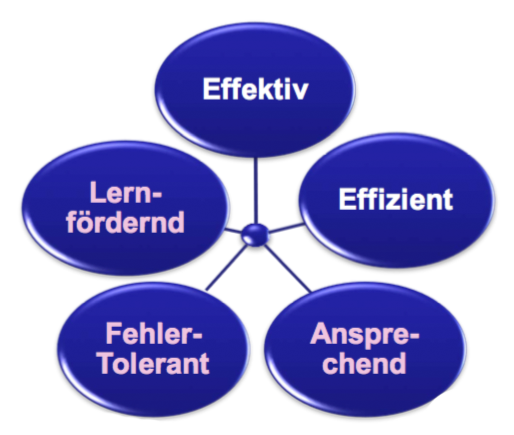
\includegraphics[width=0.120\textwidth]{images/usability-11}
 \columnbreak
 \textbf{ Effektivität:}
Benutzer können ihre Ziele erreichen
\textbf{ Effizienz: }
Benutzer können ihre Ziele mit angemessenem Aufwand erreichen
\textbf{Zufriedenheit:}
Benutzer sind positiv gegenüber dem System eingestellt
\end{multicols}

\subsubsection{Prinzipien der Dialoggestaltung (ISO 9241-110)}

\textbf{Aufgabenangemessenheit}
Benutzer erledigen Aufgaben effektiv und effizient
\textbf{Selbstbeschreibungsfähigkeit}
Dialogschritte sind durch Beschreibungen oder Rückmeldungen verständlich oder werden erklärt
\textbf{Steuerbarkeit}
Benutzer kann Richtung und Geschwindigkeit der Interaktion beeinflussen
\textbf{Erwartungskonformität}
Dialog entspricht den Kenntnissen des Benutzers
\textbf{Fehlertoleranz}
Trotz erkennbar fehlerhafter Eingaben des Benutzers kann das Ziel effizient erreicht werden
\textbf{Individualisierbarkeit}
Interaktion kann angepasst werden
\textbf{Lernförderlichkeit}
Erlernen der Anwendung wird unterstützt
\subsubsection{Stone et al. 2005}
\textbf{Visibility:} Der erste Schritt zum Ziel ist sichtbar
\textbf{Affordance:} (Begreifbarkeit) Aktionsresultat ist vorhersagbar
\textbf{Feedback:} Es ist klar was passiert ist (oder passiert -> Animation)
\textbf{Simplicity:} Nicht mehr als nötig für die Aufgabe
\textbf{Structure:} Logische und konsistente Organisation
\textbf{Consistency:} Vorhersagbarkeit durch Konsistenz
\textbf{Tolerance:} Fehler vermeiden, Wiederherstellung vereinfachen
\textbf{Accessibility:} Design für alle Personengruppen \& Situationen
\subsubsection{Garret}
\textbf{Oberfläche:} konkret Attraktiv, Vertrauenserweckend, .. “Hedonische Qualität“
-> Graphic Design
\textbf{Raster:} Erwartungskonform, Fehlertolerant, Effizient -> Interaktionsdesign mit Wireframes
\textbf{Struktur} Aufgabengerecht, Fehlertolerant, Effizient
-> Interaktionsdesign mit Szenarios -> Informationsarchitektur
\textbf{Umfang} Zielgruppengerecht, Effektivität -> Anforderungsanalyse, Ziele, Aufgaben
\textbf{Strategie}  Marktgerecht-> Marktanalyse, Zielgruppenanalyse
%Usability
%UCD
\subsubsection{UCD}
\begin{multicols}{2}
\subsubsection{Cognitive Walktrough / Usability Testing}
\tiny Ist eine je Methode zur Identifikation von Usability Problemen. Cognitive 
Walktrough wird durchgeführt von 3 oder mehr Experten und Usability Testing 
von 3 oder mehr zukünftigen Nutzer. Für Usability Testing braucht es noch kein 
lauffähiges System, Screenshots reichen. Grösste Herausforderung bei Usability 
Testing ist die Erstellung guter Aufgaben, bei welchen echte Benutzerziele getestet 
werden ohne, dass Keywords verraten werden.
\subsubsection{User Centered Design}
Elemente der User Experience: Oberfläche (Aufmerksamkeiten, 
Erkennung von Bekanntem), Raster (Responsive Design), Struktur (Usability), 
Umfang, Strategie.
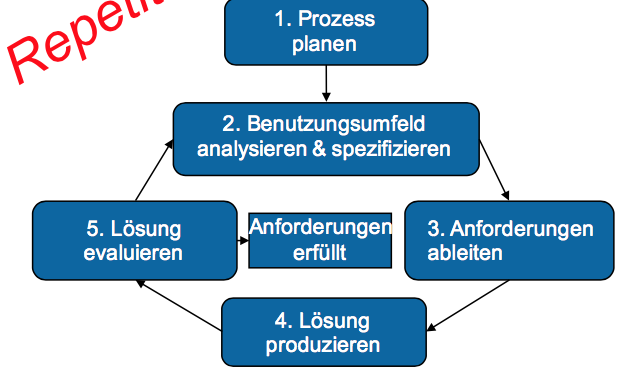
\includegraphics[width=0.12\textwidth]{images/ucd}
\end{multicols}
%UCD
\subsubsection{JS}



\subsubsection{Template Engine}


\end{multicols*}
\end{document}